\documentclass[draft]{agujournal2018}
\usepackage{url}
\usepackage[utf8]{inputenc}
\usepackage{amsmath}
\usepackage{rotating}
\usepackage{multirow}
\usepackage{booktabs}
\usepackage[font=normalsize]{caption}
\usepackage[flushleft]{threeparttable}
\journalname{JGR: Solid Earth}

\linenumbers

\usepackage{ragged2e}

\usepackage{apacite}
\usepackage{url}

\author{Kelian Dascher-Cousineau}

\begin{document}
\large
\title{What controls variations in aftershock productivity?}

\authors{Kelian Dascher-Cousineau, Emily E. Brodsky, Thorne Lay}


% \affiliation{1}{First Affiliation}
% \affiliation{2}{Second Affiliation}
% \affiliation{3}{Third Affiliation}
% \affiliation{4}{Fourth Affiliation}

\affiliation{}{University of California Santa Cruz, 1156 High Street
Earth and Planetary Sciences, Santa Cruz, CA 95064}
%(repeat as many times as is necessary)

%% Corresponding Author:
% Corresponding author mailing address and e-mail address:

% (include name and email addresses of the corresponding author.  More
% than one corresponding author is allowed in this LaTeX file and for
% publication; but only one corresponding author is allowed in our
% editorial system.)

% Example: \correspondingauthor{First and Last Name}{email@address.edu}

\correspondingauthor{Kelian Dascher-Cousineau}{kdascher@ucsc.edu}

%% Keypoints, final entry on title page.

%  List up to three key points (at least one is required)
%  Key Points summarize the main points and conclusions of the article
%  Each must be 100 characters or less with no special characters or punctuation

% Example:
% \begin{keypoints}
% \item	List up to three key points (at least one is required)
% \item	Key Points summarize the main points and conclusions of the article
% \item	Each must be 100 characters or less with no special characters or punctuation
% \end{keypoints}


\begin{keypoints}
\item Lithosphere age, plate boundary type, normalized rupture area, aspect ratio, and dip significantly influence aftershock productivity.
\item Flexible multi-attribute models improve aftershock hazard prediction.
\item The volume of available brittle lithosphere appears to be the primary control on aftershock productivity.
\end{keypoints}

\newpage

\justify

\section*{Abstract}

Earthquake aftershocks are nearly ubiquitous. The number of aftershocks increases with mainshock size following a well-defined scaling law. However, excursions from the average behavior are common. This variability is particularly concerning for large earthquakes where the number of damaging aftershocks varies by a  factor of 40 for mainshocks of comparable magnitude. Do observable factors lead to differences in aftershock behavior? We examine aftershock productivity relative to the global average for all mainshocks ($M_W>6.5$) from 1990 to 2019. A global map of earthquake productivity highlights the influence of tectonic regimes. From a suite of factors related to regional setting, we find that earthquake depth and lithosphere age correlate with earthquake productivity. We investigate the role of source attributes by compiling source dimensions, radiated seismic energy, new measurements of stress drop, and a novel measure of slip heterogeneity based on finite fault source inversions for the largest earthquakes from 1990 to 2017. Particularly long and narrow, and high stress drop ruptures have lower productivity. A machine learning method shows that a particular set of parameters (dip, lithospheric age and normalized rupture area) combine well to improve predictions of aftershock productivity on a cross-validated data set. Our overall analysis is consistent with a model where the volumetric abundance of nearby stressed faults controls the aftershock productivity rather than variations in source stress. The insights from this study shed light on a complementary approach to predicting relative productivity based on geological and rupture properties rather than empirical calibration.  

\section{Introduction}

Earthquakes cluster in time and space. In a typical sequence, the largest earthquake is the mainshock, those preceding are foreshocks, and those following are aftershocks \citep{Omori1895}. The clustering behavior is well-described by a small set of statistical laws \citep[e.g.,][]{Ogata1988}. For instance, the aftershock productivity law, which is sometimes known as the Reasenberg-Jones Law is

\begin{linenomath*}
\begin{equation}\label{eq:productivity}
    N(M)=k10^{\alpha M}
\end{equation}
\end{linenomath*}

where $N$ is the number of aftershocks, $M$ is the mainshock magnitude, and $k$ is a constant of proportionality which subsumes the tendency to generate aftershocks and the magnitude of completeness of the earthquake catalog. The productivity law fits a wide range of data with $\alpha\approx1$ \citep{Reasenberg1989, Yamanaka1990scalingshock,  DeArcangelis2016, Kisslinger1996,Tahir2015,Tahir2014Aftershock2005, Page}. Thus the basic phenomenon of an increasing number of aftershocks with increasing mainshock magnitude is captured and quantified empirically.

    \begin{figure}[!ht]
        \centering
        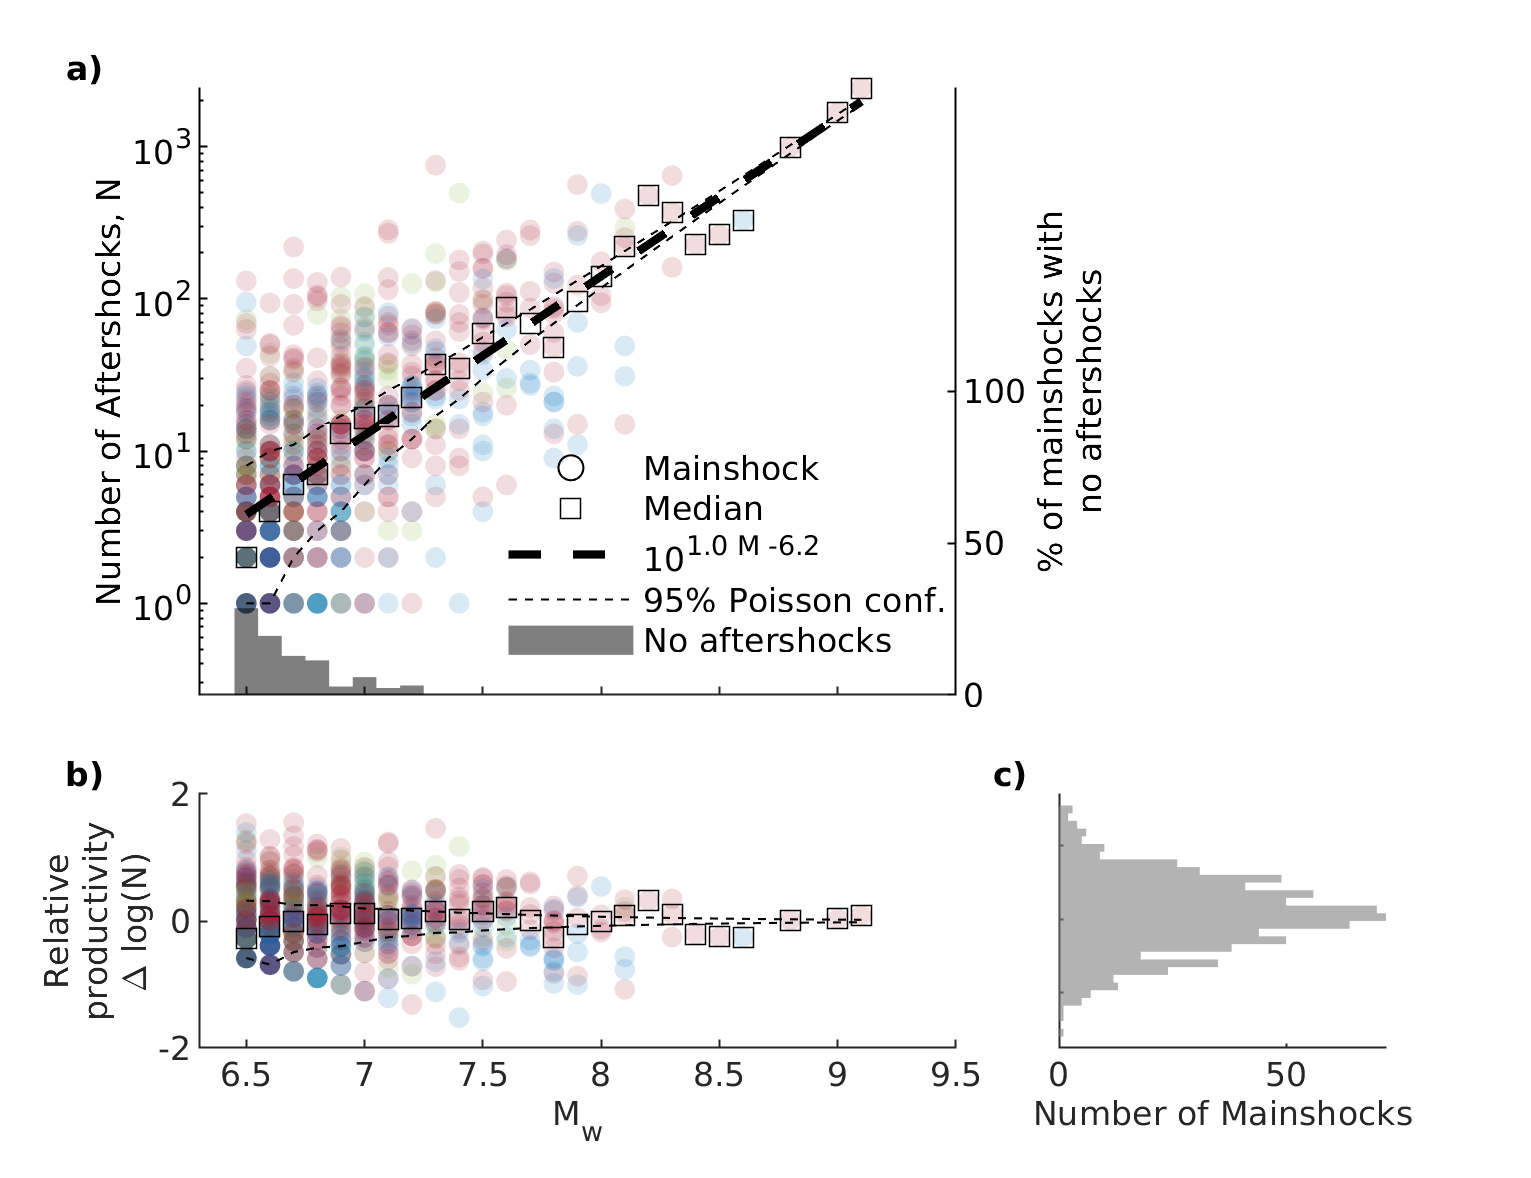
\includegraphics{figures/prod_law.png}
        \caption{a) The number of aftershocks of $M_W\ge4.5$ within three source dimensions and 60 days as a function of mainshock magnitude identified in the global ISC and NEIC catalogs from 1990 to 2019. Colors indicate faulting style of the mainshock; blue, green and red points correspond to earthquake sequences for which the mainshock was respectively strike-slip, normal or reverse. The global productivity law (dashed line) is fit using a least squares regression through the median log-number of aftershocks for each 0.1 magnitude bin (black squares). The median number includes mainshocks with no aftershocks which are not shown on the plot. Note the individual earthquake sequences (circles) exhibit significant scatter around the productivity law. b) Relative productivity (Eq.~\ref{eq:residual_productivity}) as a function of mainshock magnitude. The relative productivity distribution does not show events with no aftershocks and thus the lower left corner of the plot is underpopulated. c) Histogram of the relative productivity of mainshocks considered in this study.
        }
        \label{fig:fms_prod}
    \end{figure}

Significant variations occur relative to the productivity law. Figure \ref{fig:fms_prod}a shows 40-fold differences in the number of aftershocks for events of similar magnitude. Excursions from the scaling relationship are documented by prior work \citep[e.g.][]{Marsan2017HowAftershocks,Boettcher2004EarthquakeFaults,Page,Tahir2014Aftershock2005}. Are these variations stochastic and unpredictable, or are they determined by features of particular sites or earthquakes?

The answer has practical consequences. Aftershock forecasting is currently the only operational form of earthquake prediction and is routinely used in the wake of major earthquakes to advise on short-term hazard following an earthquake \citep{Reasenberg1989,Page}. Within a sequence, the probability of subsequent earthquakes exceeding the magnitude of the mainshock relates directly to the productivity \citep{Reasenberg1989, Reasenberg1999ForeshockEarthquakes}. Currently, variability in aftershock productivity is calibrated regionally where data permits or extrapolated from nearby regions and updated over the course of the aftershock sequence \citep[e.g.][]{Reasenberg1989, Reasenberg1999ForeshockEarthquakes, ogata2017statistics}. These forecasts are entirely physics-free and, notably, rely heavily on high quality seismic data both before and during the earthquake \citep{Gerstenberger2005Real-timeCalifornia, Omi2015Intermediate-termApproaches}.

Yet previous observers find that features related to the setting of the mainshock can inform aftershock abundance. Both global and regional studies indicate that tectonic regions have distinct aftershocks statistics \citep{Chu2011, Page, Davidsen2015GeneralizedCalifornia, Tahir2014Aftershock2005, ogata2017statistics}. For instance, the Eastern Pacific has greater aftershock productivity than the Western Pacific \citep{Singh1988Regionalle7.0, Wetzler2016}. Seismotectonic subdivisions (plate boundaries, global geology, seismicity catalogs, and regional and local studies) yield 10-fold differences in aftershocks productivity \citep{Page}. Active non-subduction continental regions have elevated earthquake productivity and, on average, larger aftershocks \citep{Page, Mogi1967, Davis1991Single-linkVariations}. In contrast, ridge transform faults are deficient in aftershocks \citep{Davis1991Single-linkVariations, Boettcher2004EarthquakeFaults, McGuire2005}. The local geological structure is thought to underlie these distinctions \citep{Boettcher2004EarthquakeFaults, McCloskey2003StructuralAftershocks}. \citet{Yamanaka1990scalingshock} report intraplate earthquakes as more productive than plate boundary earthquakes. Case studies generally reinforce the importance of geological structures on the distribution and intensity of aftershocks \citep{Das2003SpatialDistribution, McCloskey2003StructuralAftershocks}. An extreme case comes from deep focus subduction zone earthquakes, which sometimes generate few or no observable aftershocks \citep{Bath1965LateralMantle, Frohlich1989TheEarthquakes, Nyffenegger2000, Wiens1997AftershockZone, Wu1999, Houston2004}. Some work attributes the deficiency to the elevated temperature at depth \citep{Nyffenegger2000, Houston2004}. 

Other studies elucidate the importance of source effects. Theoretical arguments, supported by systematics in the variance of stress drop measurements and earthquake productivity, have suggested that increased stress drop should correspond to increased productivity for Californian seismicity \citep{Marsan2017HowAftershocks}. The opposite relationship was documented for recent (1990-2016) major megathrust ruptures ($M_W \ge 7$) \citep{Wetzler2016}. The authors suggested that high stress drop corresponds to a smaller rupture area and therefore fewer aftershocks. This is supported by a tendency for megathrust aftershocks to occur on the periphery of large-slip zones \citep{Wetzler2016}. Earthquakes rupturing at supershear velocities also appear to have low aftershock productivity \citep{Bouchon2008TheEarthquakes}. A relationship between the heterogeneity of a rupture and the number of aftershocks has been a long-standing contention \citep{Mogi1967, Yamanaka1990scalingshock} with some support from rate and state models \citep{Helmstetter2006RelationModel, Marsan2006}, but few direct and quantitative measurements \citep{Das2003SpatialDistribution, Houston2004}. Finally, occurrence of dynamic triggering would suggest that radiated energy should influence the number of aftershocks \citep{felzer2006decay}.  

Some observations cannot be distinctly associated with setting or source. There is a relationship between relative aftershock productivity and focal mechanism. Strike-slip earthquakes are proposed to be intrinsically less productive than dip-slip earthquakes \citep{Tahir2012, Tahir2014Aftershock2005, Tahir2015}. However, since strike-slip earthquakes occur in certain regions, it is unclear whether the reduced productivity is a site or source effect.

% Roadmap paragraph
The diversity in methods and data sets hinder an assessment of the relative importance of the above conclusions. The goals of this paper are to 1) systematically assess both setting and source effects on relative aftershock productivity and distill them down to a list of significant parameters, 2) examine the constraints on the physical controls of aftershock productivity and 3) outline complementary approaches for tuning seismic hazard predictions following large earthquakes. We first present a method of measuring relative aftershock productivity and defining a metric. We then provide an overview of global patterns in earthquake productivity, systematically addressing setting and source effects. We consider setting effects such as plate boundary type, depth, and lithospheric age; and source effects such as radiated energy, stress drop, source geometry, and slip heterogeneity. We attempt to disentangle site versus source focal mechanism influences using nearly co-located events. Machine learning tools establish a parsimonious set of parameters that can help in aftershock prediction and be used to improve our understanding of the physical controls on aftershock generation. Results indicate that the geometry of the source and the corresponding volumetric availability of stressed faults determine variations in earthquake productivity.

\section{Metrics and Data}
   
    \subsection{Measuring Aftershock Productivity}
    
This study requires a consistent measure of aftershock productivity comparable on a global basis. To this end, we use a space-time windowing method to identify and count aftershocks. The event-level questions focusing on variations from the mean behavior examined here do not favor methods adaptively fitting different time or space periods and other seismicity parameters \citep[e.g.][]{ogata2017statistics, Zaliapin2008}.

We classify earthquakes as foreshocks, mainshocks or aftershocks in a hierarchical sense \citep[following][]{felzer2006decay, Brodsky2011TheForeshocks, Wetzler2016}. We define the largest earthquake in the catalog as a mainshock and then mark as foreshocks and aftershocks earthquakes within magnitude-dependent space and fixed time windows before and after the mainshock. The identified foreshocks and aftershocks are removed from consideration as mainshocks to prevent double counting. A larger space and time window is used to ensure separation of sequences. Earthquakes within this larger window are also removed from consideration as potential mainshocks but do not count as aftershocks. We sequentially proceed to smaller mainshocks with this classification of foreshocks and aftershocks until we exhaust the catalog. The method is not designed to capture absolutely every aftershock, but rather to provide a consistent measure of aftershock productivity of each isolated mainshock. 

Specific trade-offs determine the choice of the time and space windows. Smaller windows increase the confidence that aftershocks are correctly attributed; conversely, larger time windows include more aftershocks and limit the effect of censored statistics (mainshocks with no aftershocks). We balance these trade-offs to find window selection criteria that yield the standard productivity relationships over the analyzed magnitude range (Figure~\ref{fig:sensitivity}). We assess the performance of each space-time window by comparing the results to the median of 100 time-shuffled catalogs that preserves the original spatial distribution but break the actual time sequence of the catalog \citep{Garza-Giron2018Mainshock-AftershockRegions}. The space-time window that includes the most aftershocks while separating the actual aftershock productivity relationship from the shuffled ones is the preferred choice.
  
Figure~\ref{fig:sensitivity} shows results for a suite of space and time windows. Space windows are all measured in terms of source dimensions estimated following \citet{Wells1994}:
\begin{linenomath*}
\begin{equation}\label{eq:wells}
    R_{source}\sim 2\times 10^{0.59M}
\end{equation}
\end{linenomath*}
For reference, $M_W$ 6 and 9 earthquakes have dimensions on the order of $\sim 7$ km and $\sim 400$ km respectively. A spherical space window of three source dimensions in radius centered on the mainshock location and a time window of 60 days following the mainshock performs best. Smaller and shorter windows result in a clearer separation of the shuffled statistic. However, the number of mainshocks with no aftershocks increases dramatically (e.g., 30\% of mainshocks in the case of the ten-day and one source dimension window, as opposed to the chosen 10\% for the our selected window). The larger space window, used to eliminate events from further consideration, is four source dimensions and an additional 40 days. We use the same combination of selection and screening in space window and 1 day time window to classify foreshocks. Using the space-time windowing approach we ensure that nearly all mainshocks (99\%) are fully isolated in time and space from each other.

\begin{sidewaysfigure}
    \centering
    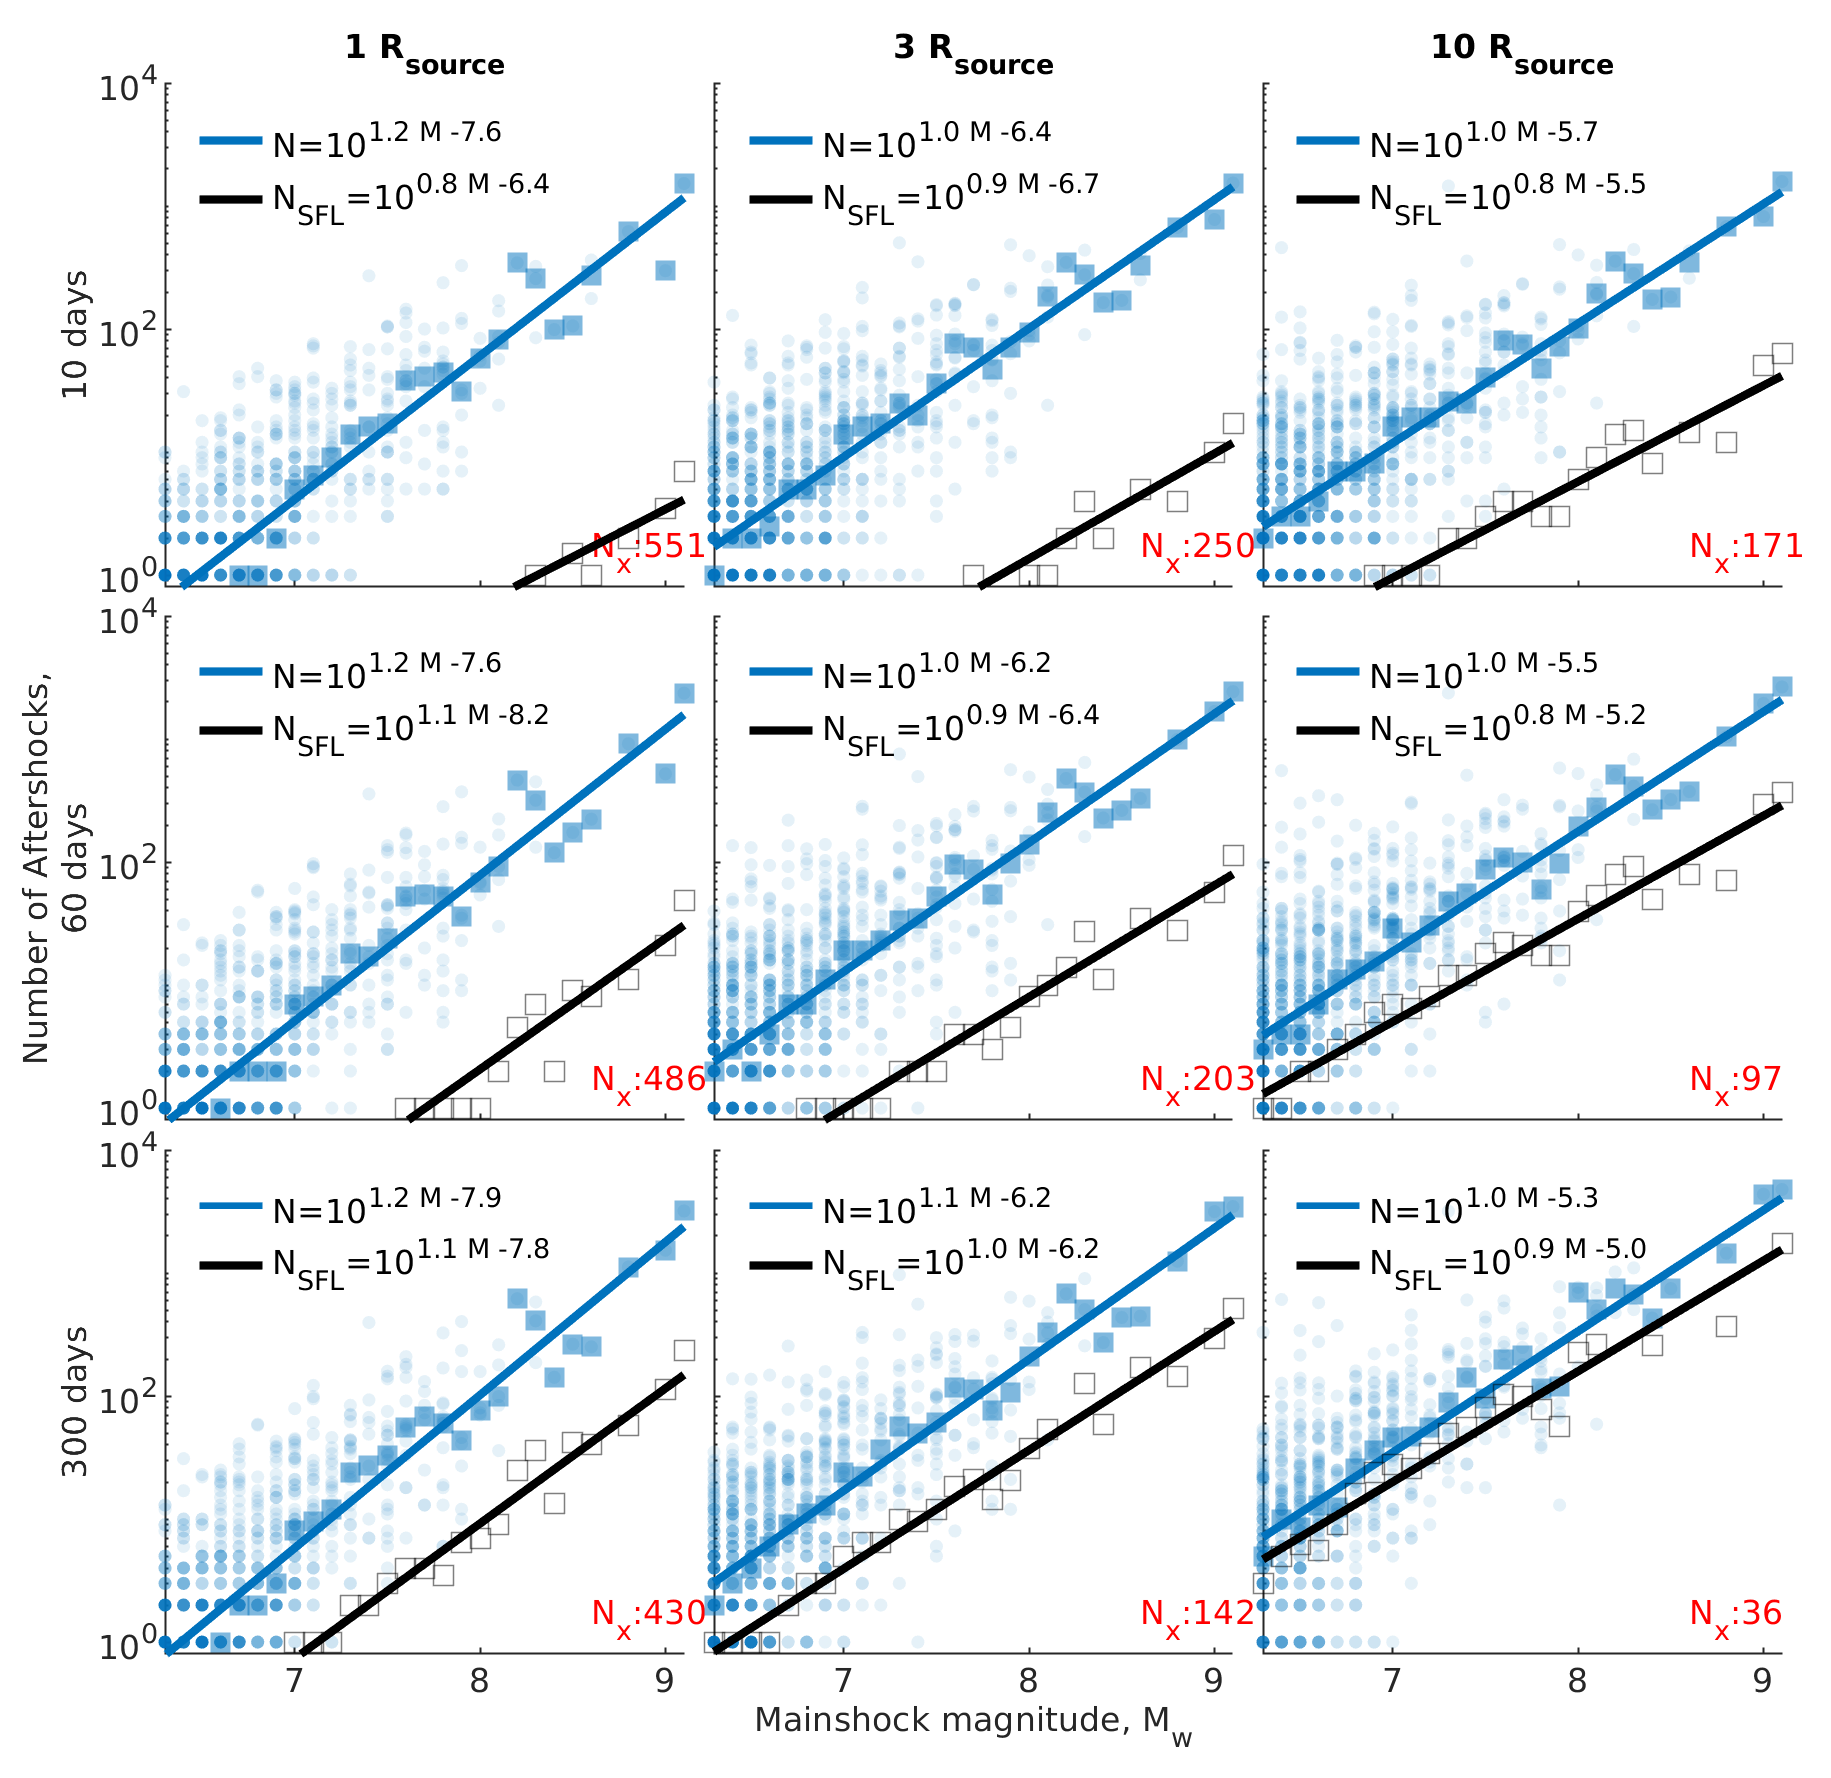
\includegraphics{figures/sensitivity.png}
    \caption{Sensitivity analysis of space-time windows. Time windows of 10, 60, and 100 days and spherical space windows with radii of 1, 3, and 10 source dimensions ($R_{source}$) are considered. Blue circles indicate the number of aftershocks and corresponding mainshock magnitude identified we our hierarchical counting routine. The blue line indicates the outcome of a regression the median log-number of aftershocks for each 0.1 magnitude bin (blue squares). For reference, we computed the same productivity relationship, $N_{SFL}$ (black line), for the median of 100 time-shuffled catalogs (grey squares). For each space-time window, we indicate the number of mainshocks with no aftershocks in red ($N_x$). Note that as space and time windows increase, more mainshocks have measurable aftershock counts. However, the likelihood of counting background productivity and significantly affecting subsequent parameterization becomes an increasing concern.
}
    \label{fig:sensitivity}
\end{sidewaysfigure} 


We compute the median number of aftershocks for each 0.1 magnitude bin in the mainshocks catalog (including the counts of events with zero aftershocks) and the corresponding magnitude to perform a linear least squares inversion and determine the $k$ and $\alpha$ (Figure \ref{fig:fms_prod}a). Using these parameters, we define the relative productivity ($\Delta \log(N)$) for each mainshock as 
%
\begin{linenomath*}
\begin{equation}{\label{eq:residual_productivity}}
    \Delta \log(N) = log(N) - log(\hat{N}(M)) = log\left(\dfrac{N}{k10^{\alpha M}}\right)
\end{equation}
\end{linenomath*}
%
where $N$ is the number of aftershocks following a mainshock and $\hat{N}(M)$ is the number of aftershocks predicted for the mainshock magnitude, $M$, from Equation \ref{eq:productivity}. The relative productivity takes into account the effect of magnitude allowing us to study other factors leading to aftershock abundance (Figure \ref{fig:fms_prod}b-c). We use the relative productivity extensively throughout this study. 

\subsection{Earthquake Catalogs and Investigated Parameters}

We measure the relative aftershock productivity for mainshock magnitudes exceeding $M_W6.5$ using the National Earthquake Information Center (NEIC) for recent events and the International Seismological Center (ISC) locations and magnitudes when they become available for events form 1990 to 2019 with moment magnitude exceeding an estimated global catalog completeness, $M_W4.5$, as determined by the first local minimum of a Kolmogorov-Smirnov test. Supplement Figures S1 to S11 reproduces this study's results using a more conservative completeness estimate of $M_W5$. 

We compare relative aftershock productivity to attributes that include site effects and source effects. Table \ref{tbl:attributes} outlines the selected attributes, coverage, and corresponding data sources. Locations, focal mechanism solutions, and radiated energy estimates were all obtained from the Incorporated Research Institutions for Seismology (IRIS) data management center and merged using earthquake identification numbers. Finite fault inversions produced and cataloged by \citet{Hayes2017} were associated with an aftershock statistic using a standardized Euclidean distance ($M_W$, latitude, longitude, depth, time).
Data and analytical limitations are such that rupture properties and source geometry are only available for 98 mainshocks. Supplement Table S1 \citep{Hayes2017} includes the source attributes for these mainshocks. We treat multi-segmented rupture separately.

Certain measures in the table require a specific explanation. We remove any magnitude dependence to source attributes by scaling and log-transforming source attributes. Accordingly, radiated energy is normalized to moment; width and length are normalized by standard scaling dimensions (Equation \ref{eq:wells}); and the rupture area is likewise normalized to the squared value of standard source dimensions. All are then log-transformed to linearize their distribution. 

Following recommendations of \citet{Noda2013}, we compute stress drop measurements for all single plane finite fault inversions. Smoothing constraints on the finite fault inversions imply that the stress drop measurements are likely a lower, but consistent bound \citep{Adams2017ExploringInversions}. 

Finally, we introduce a novel quantification of slip heterogeneity ($H$) derived from finite fault inversions. The metric compares the observed slip to a smooth reference slip distribution,
%
\begin{linenomath*}
\begin{equation}
    H = \dfrac{\mu \int_\Sigma |u-u_{ref}| dS}{M_o},
\end{equation}
\end{linenomath*}
%
where $\mu$ is the shear modulus, $u$ is the observed slip distribution, $u_{ref}$ is the reference slip distribution, $dS$ is an area element on the fault, $\Sigma$ is the entire finite fault area, and $M_o$ is the earthquake moment. The reference slip is prescribed as a positive ellipsoid fit to the slip distribution defined by free parameters $u_{c}, x_0, y_0, a$ and $b$,
%
\begin{linenomath*}
\begin{equation}\label{eq:heterogeneity}
u_{ref}=\left\{
\begin{array}{@{}ll@{}}
     \sqrt{u_{c}^2 - \left(\dfrac{x-x_0}{a}\right)^2 +  \left(\dfrac{y-y_0}{b}\right)^2}, & \text{if}\ \left(\dfrac{x-x_0}{a}\right)^2 +  \left(\dfrac{y-y_0}{b}\right)^2 < 1 \\
     \\
    0, & \text{otherwise}
    \end{array}\right.
\end{equation}
\end{linenomath*}

The heterogeneity measurement is designed to be most sensitive to large slip fluctuations such as asperities or barriers.

\begin{table}[]
\caption{Attributes featured in this study.}
\label{tbl:attributes}

\begin{threeparttable}
\centering
\setlength{\tabcolsep}{5.5pt}
\renewcommand{\arraystretch}{1.3}
\linespread{0.5}\selectfont\centering

\begin{tabular}{@{}lp{2cm}p{1cm}ccp{6.5cm}@{}}
\toprule
          & \textbf{Attributes}             & \multicolumn{3}{c}  {\textbf{Coverage}}  & \textbf{Comments}                                                                                                                                                                                          \\ \cmidrule(lr){3-5}
          &                                 & Spatial      & $M_c$ & Mainshocks  &                                                                                                                                                                                                            \\ \midrule
\multicolumn{2}{l}{\textbf{Site effects}}   &              &       &      &                                                                                                                                                                                                            \\
          & Time-location\tnote{1}          & Global       & 4.5   & 1011 &                                                                                                                                                                                                            \\
          & Plate boundaries\tnote{2}       & Global       & -     & 1011 & Categorized by nearest digitized boundary provided the focal mechanism is congruent\tnote{7} \hspace{1mm} for earthquakes $<$ 400 km from plate boundary; others are intraplate.                                                \\
          & Plate age and velocity\tnote{3} & Ocean basins & -     & 268  & Determined by nearest crustal age measurement up to 30 km from the mainshock.                                                                                                                                  \\
        %   & Lithospheric thickness\tnote{4} & Global       & -     & 2662 &                                                                                                                                                                                                            \\
\multicolumn{2}{l}{\textbf{Source effects}} &              &       &      &                                                                                                                                                                                                            \\
          & Radiated Energy\tnote{5}        & Global       & 6.0   &      &                                                                                                                                                                                                            \\
          & Source dimensions\tnote{6}      & Global       & 7.0   & 98   & Width (along-dip), length (along-strike) and aspect ratio of ruptures determined from autocorrelation width of finite fault inversions \citep[following][]{mai2000}. See text for notes on scaling.                                 \\
          & Rupture duration and velocity\tnote{7}& Global  & 7.0   & 98   &                                                                                                                                                                                                            \\
          & Material properties\tnote{7}    & Global       & 7.0   & 98   & $V_p$, $V_s$ and density used for inversions                                                                                                                                                         \\   
          & Stress drop\tnote{6}            & Global       & 7.0   & 98   & See text                                                                                                                                                                                                  \\
          & Heterogeneity\tnote{6}          & Global       & 7.0   & 98   & See text, Equation \ref{eq:heterogeneity}                                                                                                                                                                                                   \\
\multicolumn{2}{l}{\textbf{Mixed effects}}  &              &       &      &                                                                                                                                                                                                            \\
          & Faulting style\tnote{8}         & Global       & 5.5   & 1011 & Categorized as strike-slip, normal, and reverse using the P and T axes                                                                                                                                     \\ \midrule
          &                                 &              & Total & 1011 &                                                
\end{tabular}%

    \begin{tablenotes}
        \item[1] National Earthquake Information Center (NEIC) and International Seismological Centre (ISC) catalogs downloaded from the Incorporated Research Institutions for Seismology (IRIS) data management service. 
        \item[2] \citet{Bird2003AnBoundaries}
        \item[3] \citet{Muller2008}
        % \item[4] \citet{Pasyanos2014LITHO1.0:Earth}
        \item[4] Produced by \citet{Convers2011GlobalMid2010} and downloaded from the Incorporated Research Institutions for Seismology (IRIS) data management service.
        \item[5] Attributes were derived from finite fault inversions produced by \citet{Hayes2017}.
        \item[6] Attributes directly measured by \citet{Hayes2017}.
        \item[7] Harvard global Centroid Moment Tensor Solutions (gCMT) and National Earthquake Information Center (NEIC) focal mechanism solutions downloaded from the Incorporated Research Institutions for Seismology (IRIS) data management service.

    \end{tablenotes}

\end{threeparttable}

\end{table}
%%%%%%%%%%%%%%%%%%%%%%%%%%%%%%%%%%%%%%%%%%%%%%%%%%%%%%%%%%%%%%%%%%%%%%%%%%%%%



\section{Results}
    \subsection{The Global Earthquake Productivity Map}\label{sec:glob}
    
    Our analysis yields 1011 earthquake sequences with mainshocks exceeding $M_W>6.5$. We map the global catalog of aftershock productivity (Figure \ref{fig:global_res}). We highlight characteristic global patterns which we will examine in more detail in the following sections.
    
    \begin{sidewaysfigure}
    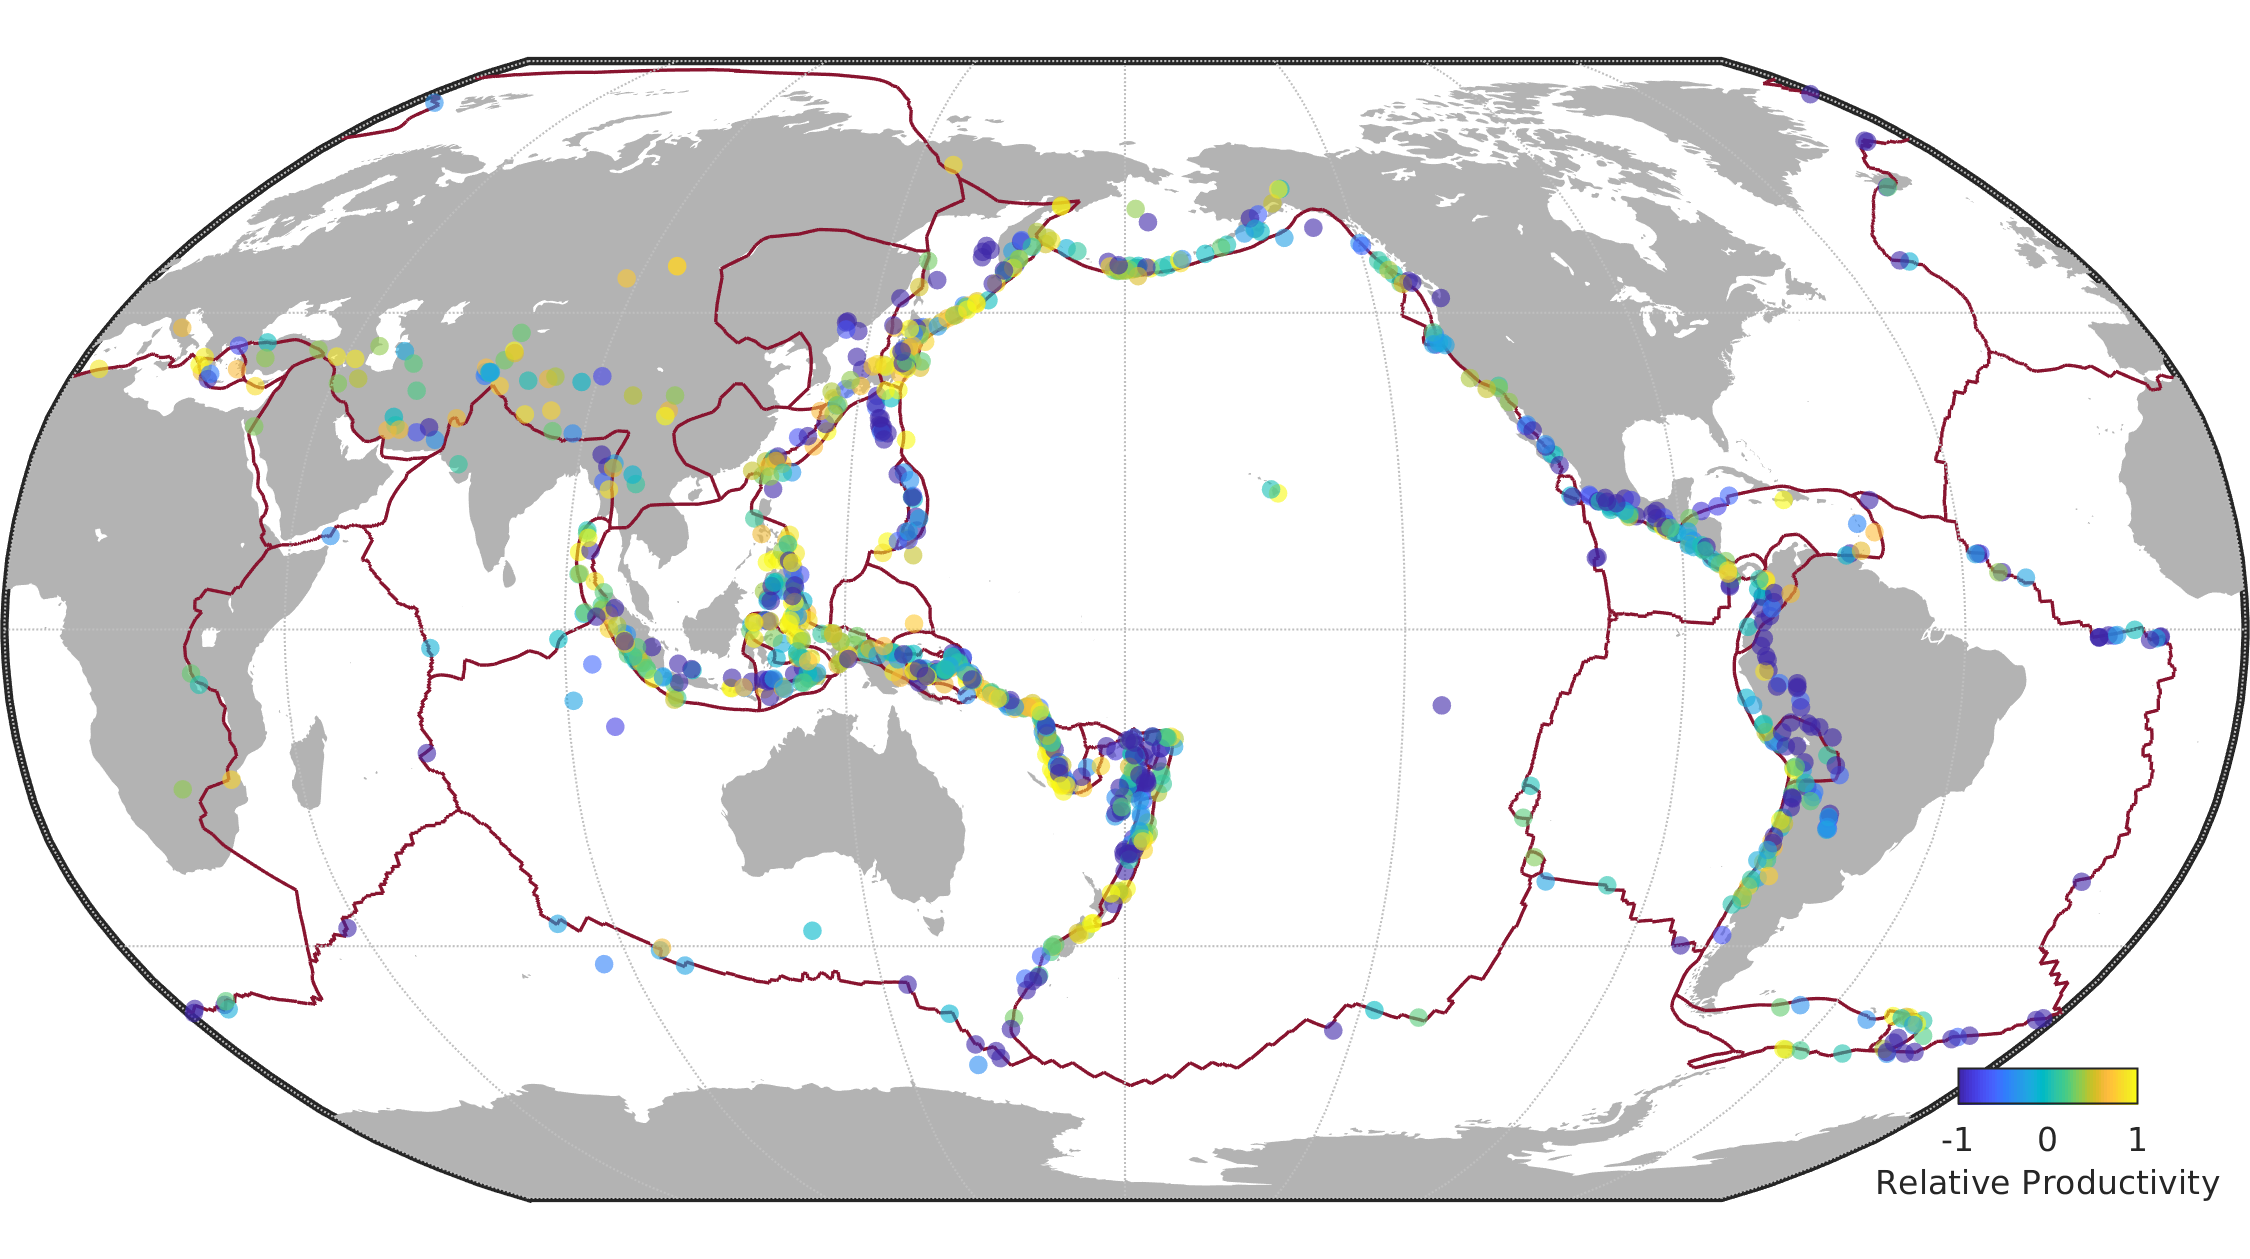
\includegraphics{figures/worldmap_res.png}
        \caption{Global map of earthquake productivity. Red lines indicate the surface trace of the tectonic boundaries. Mainshocks with $M_W\ge6.5$ color-coded according to their relative productivity (Equation \ref{eq:residual_productivity}).
        } 
        \label{fig:global_res}
    \end{sidewaysfigure}

    Intermediate- and deep-focus earthquakes stand out in the relative productivity map. Continental-scale bands of earthquakes with low relative productivity run along the Atacama, Japan, Izu-Ogasawara, Mariana and Tonga trenches. These are predominantly normal and reverse earthquakes rupturing intermediate- to deep-focus seismic zones. Over the entire catalog, earthquakes deeper than $\sim55$ km exhibit decreasing relative productivity with increasing depth (Figure \ref{fig:prod_vs_depth}). Similar observations are well documented \citep{Bath1965LateralMantle, Frohlich1989TheEarthquakes, Nyffenegger2000, Wiens1997AftershockZone, Wu1999, Houston2004}. We, therefore, do not include mainshocks deeper than 55 km  in the following analysis to avoid confounding depth with other influences.
    
    \begin{figure}
        \centering
        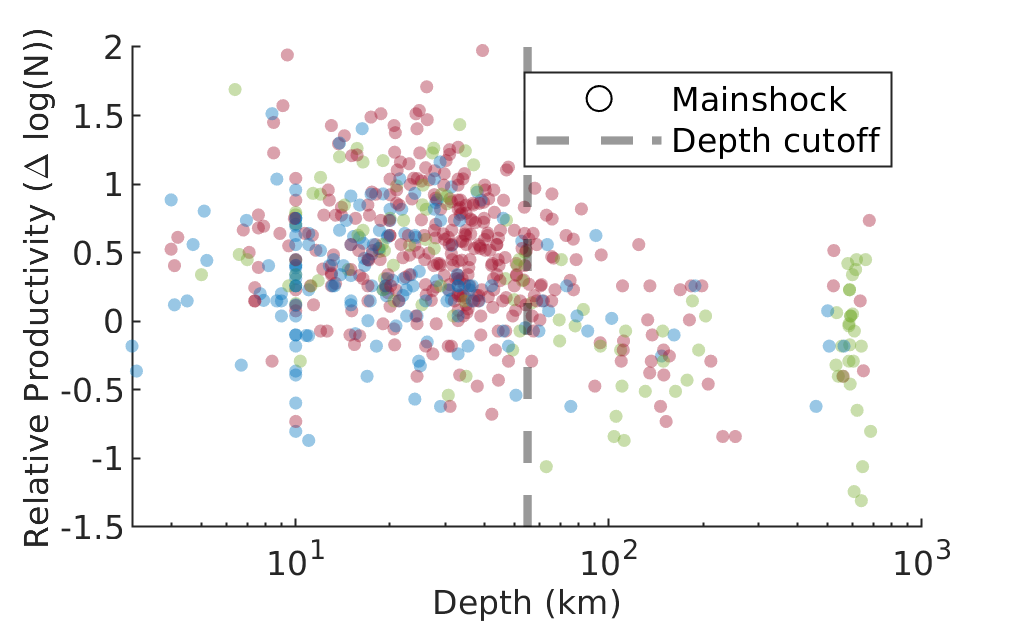
\includegraphics{figures/prod_vs_depth.png}
        \caption{Relative aftershock productivity as a function of depth. Subsequent analysis will only consider earthquakes shallower than the 55 km cutoff (dashed line). Sequences are color-coded according to faulting style of the mainshock (blue: strike-slip, green: normal and red: reverse).
        }
        \label{fig:prod_vs_depth}
    \end{figure}
    
    Offshore earthquakes that are not in subduction zones have lower relative productivity. Oceanic transform and divergent boundaries usually host less productive aftershock seismicity than the global trend ($\Delta \log(N)<0$). Consider for example the 2018 $M_W7.5$ earthquake north of Honduras rupturing the Swan Islands oceanic transform fault. It had 2 aftershocks with $M_W>4.5$ within 150 km of the epicentral location; for reference, the global median aftershocks count for mainshocks of $M_W7.5$ is 11 and therefore $\Delta log(N) = -0.7$. Earlier earthquakes along the transform have similarly low relative productivity. There are very few productive offshore earthquakes. The $M_W8.6$ 2012 intraplate strike-slip rupture offshore Sumatra followed by a $M_W8.2$ aftershock appears to be among the most productive earthquakes hosted in oceanic lithosphere not within a convergent boundary.
    
   The western coastline of North America hosts spatially coherent patterns in relative aftershock productivity (Figure \ref{fig:region}a). The Aleutian Arc grades from earthquakes with generally high aftershock productivity in the West to low aftershock productivity in the East. Earthquakes on the Queen Charlotte Fault exhibit aftershock abundances similar to the global average. Offshore clusters of seismicity along the Blanco Fracture Zone and the Mendocino Triple Junction have low productivity. Continental earthquakes along the San Andreas Fault System are markedly more productive than the seismicity to the north and south. The pronounced decrease in productivity at the southern terminus corresponds to a shift from generally transpressional continental- to transtensional oceanic-tectonics. Subduction of the northernmost section of the Cocos plate under Mexico is associated with low aftershock productivity. The number of aftershocks increases southward along central America. The gradational increases in productivity along the Aleutian Arc (westward) and Cocos Subduction zone (northward) correspond to increasing lithospheric age of the oceanic plate (Figure \ref{fig:region}b).

    \begin{figure}
        \centering
        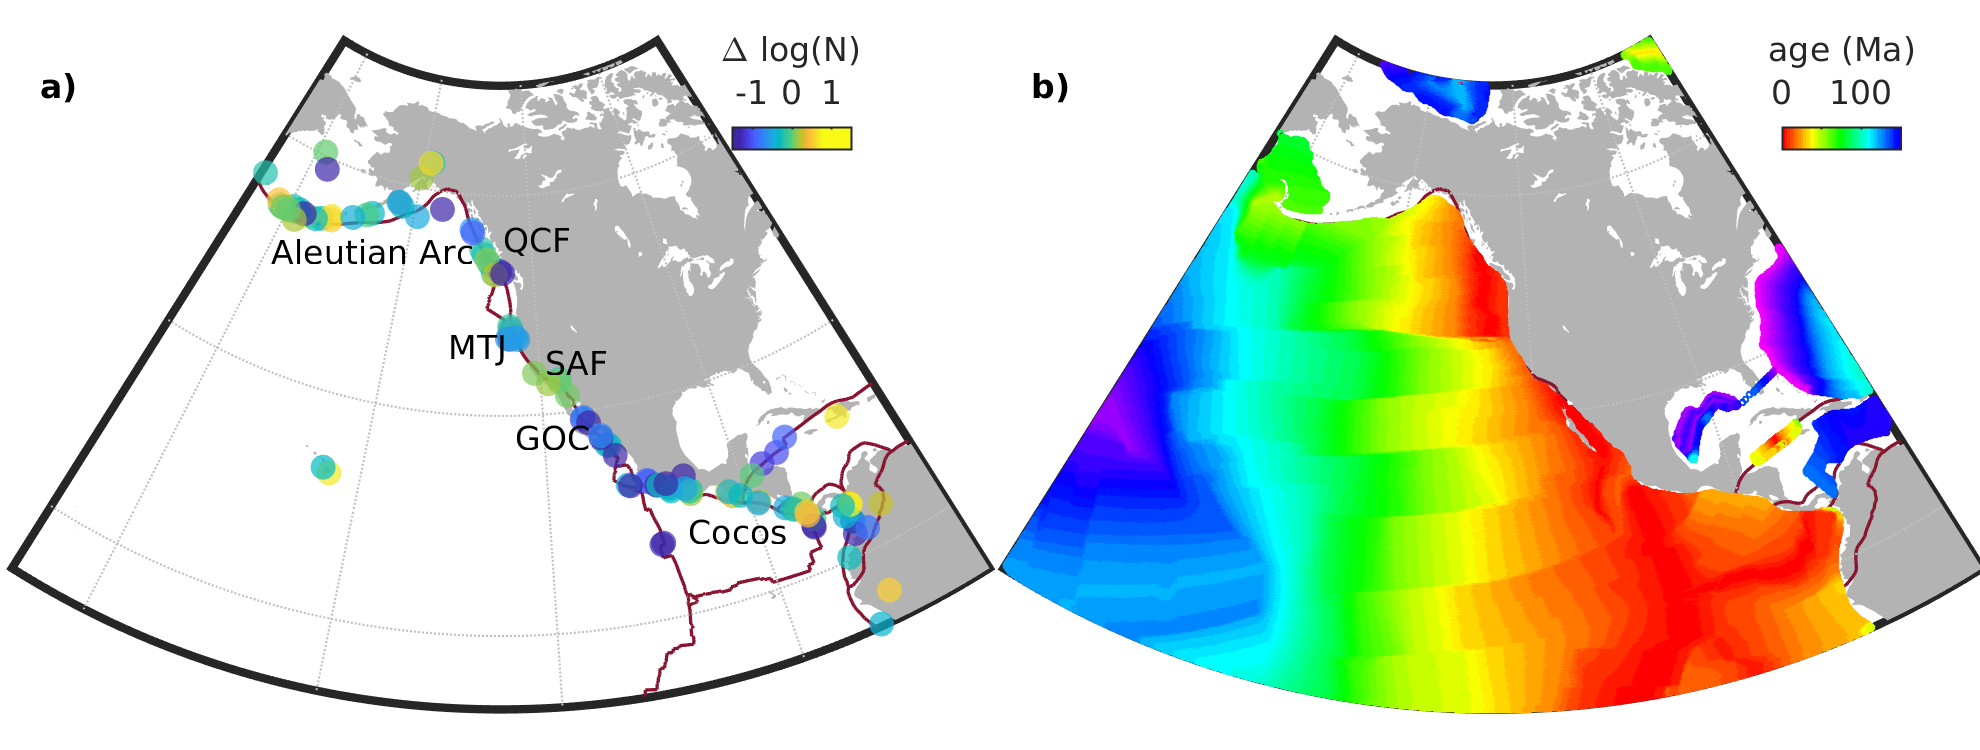
\includegraphics[width = \linewidth]{figures/regions.png}
        \caption{a) Aftershock productivity along the North American coastline.  Individual mainshocks (circles) are color-coded according to their relative aftershock productivity ($\Delta \log(N)$, Equation \ref{eq:residual_productivity}). The Aleutian Arc, Queen Charlotte Fault (QCF), Mendocino Triple Junction (MTJ), San Andreas Fault (SAF), Gulf of California (GOC) and Cocos Plate Subduction Zone include areas with coherent productivity. Red line indicates major plate boundaries \citep{Bird2003AnBoundaries}. b) Seafloor crustal age estimates from \citet{Muller2008}.}
        \label{fig:region}
    \end{figure}
    
    Continental seismicity has elevated aftershock productivity. Most notable is the India-Asia Collision Belt. Other examples include onshore seismicity in New-Zealand, the San Andreas Fault, and the Arabian Plate collision.
    
    \subsection{Tectonic Setting Effects}\label{sec:tectonic_setting}
    
    We investigate the effect of the seismo-tectonic setting on the productivity of earthquake sequences. Specifically, we subdivide the mainshock catalog by plate boundary following the categorization detailed in Table \ref{tbl:attributes}. This comparison is shown in Figure \ref{fig:plate_boundary}. The results single out oceanic transform faults as particularly deficient in aftershocks. Continental transform faults, are more productive, but less so than the global average. Subduction zones, continental convergent boundaries, continental rift basins, and oceanic convergent boundaries have similar and generally elevated relative productivity. A Kolmogorov\-Smirnov test suggests that the relative productivity of events on oceanic transform faults and continental convergent boundaries have small probabilities, $1/10^9$ and $3/10^4$ respectively, of being sampled from the overall distribution by chance; the remainder of the subsets are not significantly different from the overall distribution ($p = 0.05$ or, equivalently, a  $1/20$ chance).
    
    \begin{figure}
        \centering
        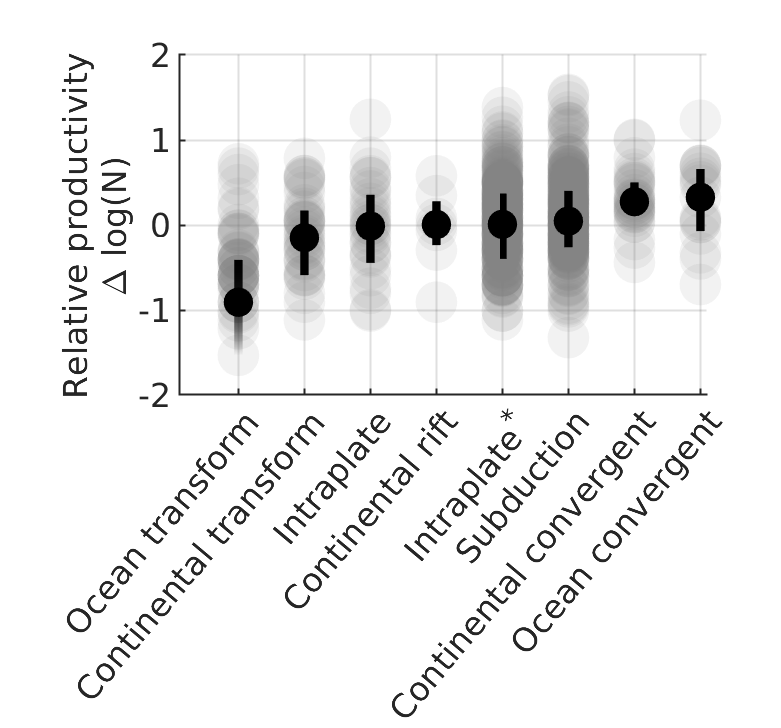
\includegraphics{figures/prod_by_pb.png}
        \caption{Earthquake productivity by tectonic boundary. Circles indicate the relative productivity of individual sequences. Solid markers and error bars indicate the median and the interquartile range. A faded lower error bar implies that mainshocks with no aftershocks are within the interquartile range. Intraplate$^*$ indicates earthquakes within 400 km of a plate boundary but with a faulting mechanism discordant with the plate boundary (e.g., outer rise events).}
        \label{fig:plate_boundary}
    \end{figure}
    
    Earthquake productivity is also related to the age of the lithosphere  (Figure \ref{fig:prod_vs_age}). Earthquake sequences in younger oceanic lithosphere tend to have fewer aftershocks. Considering all mainshocks, we observe a more systematic increase in median productivity for earthquake sequences in oceanic lithosphere less $\sim 40$ Ma in age. Strike-slip mainshocks best define the trend. Consistent with the trend, earthquakes with no aftershocks are strongly biased to oceanic lithosphere with young ages; within $<$40 Ma oceanic lithosphere, the fraction of mainshocks with no aftershocks is approximately twice as large than the global average. Performing the same analysis using a more conservative magnitude of completeness of $M_W5$ yields the same behavior, thus ensuring that the trend is not an artifact of instrumentation and catalog completeness (supplement Figure S7).
    
    \begin{figure}
        \centering
        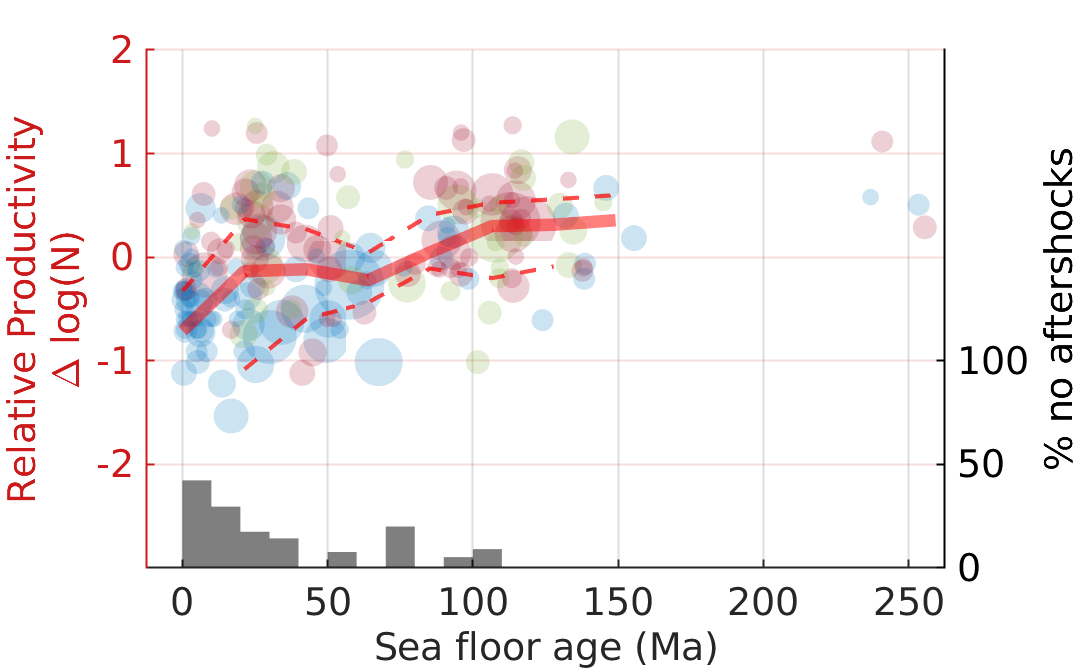
\includegraphics{figures/prod_vs_age.png}
        \caption{Relative productivity increases as a function of the age of the oceanic lithosphere. Each circle indicates an individual earthquake sequence. Sequences are color-coded by faulting style of the mainshock (blue: strike-slip, green: normal and red: reverse). The red line indicates the median average for 20Ma crustal age bins. Dashed lines indicate the corresponding interquartile ranges. Bars indicate the fraction of earthquakes with no aftershocks within each 10Ma crustal age bin.}
        \label{fig:prod_vs_age}
    \end{figure}
    
    \subsection{Source Effects}\label{sec:source_parameters}

    To identify mainshock source effects that may influence relative aftershock productivity, we linearly regress each available parameter with the relative productivity. The variance reduction for each regression is presented in Figure \ref{fig:r2_finite_fault}a. To assess statistical significance and guard against spurious correlations, we perform the same regression routine and report the maximum correlation for 10000 random permutations of the catalog with all attributes under consideration. This family-wise test serves as a robust and conservative null hypothesis. Comparing our results to the randomly shuffled realizations of the data yields the probability of obtaining equally good or better results by chance (p-values).
    
    The rupture's normalized energy, normalized length, normalized area, Poisson's Ratio, log-heterogeneity, Young's Modulus, and velocity all do not yield statistically significant linear regressions with relative productivity. Refer to the supplement (Figure S12) to see all correlations \citep{Convers2011GlobalMid2010, Hayes2017}.

    Our analysis suggests that correlations with log-stress drop and normalized width are mar\-gi\-nally significant, and that slip-zone aspect ratio is related to relative productivity in a statistically significant sense. Aftershock productivity negatively correlates with the logarithm of stress drop and aspect ratio, and positively correlates with normalized rupture width (see Figure  \ref{fig:r2_finite_fault}b-d).
    
    \begin{figure}
        \centering
        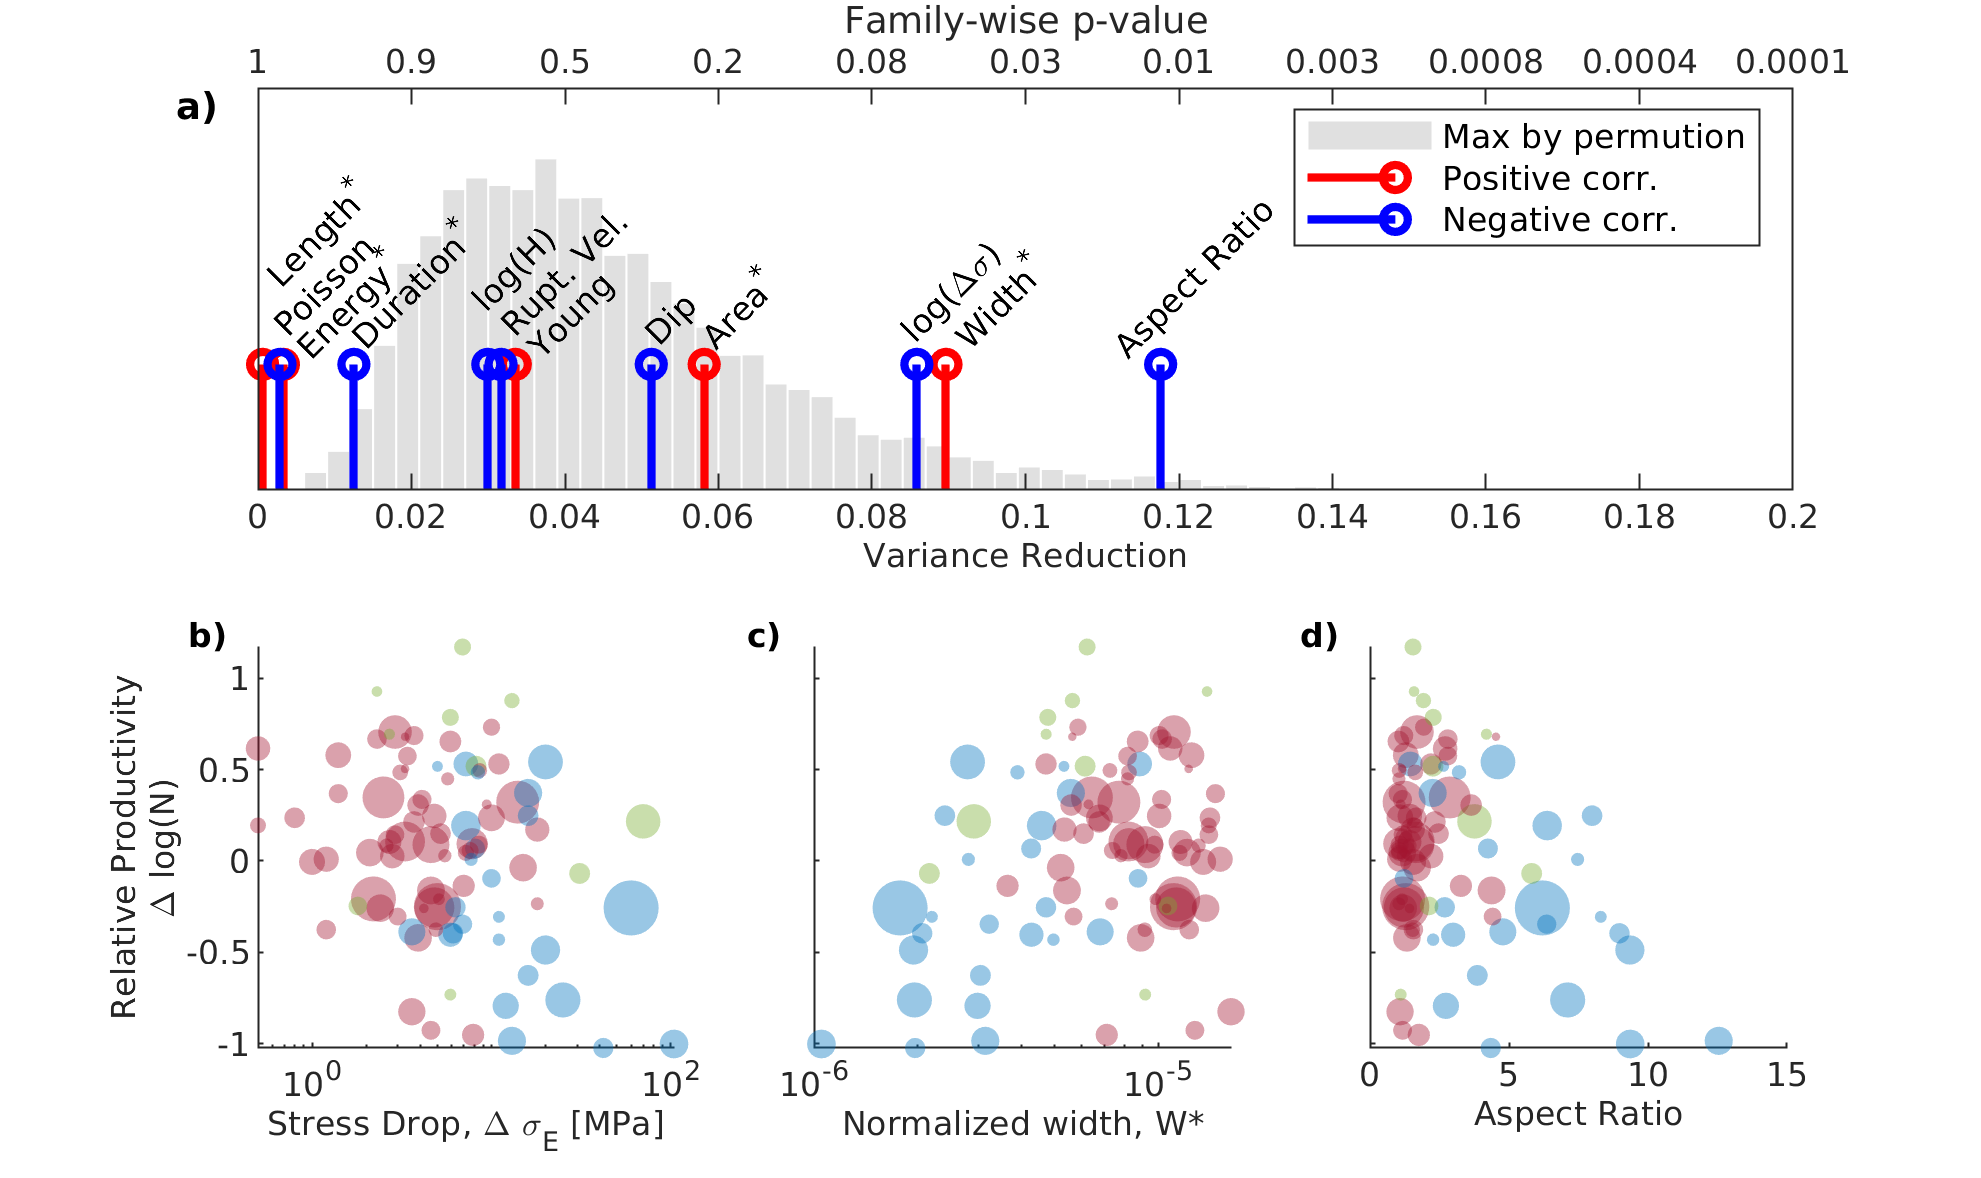
\includegraphics[width = \linewidth]{figures/stem_plot.png}
        \caption{a) Goodness of fit of linear regressions for each source attribute in our combined catalog. Top and bottom axes respectively represent the p-value and goodness of fit of each attribute (stems). The probability distribution function in the backdrop indicates the maximal variance reduction outcome of 10000 permutation test of the entire data set we tested. Asterisks indicate scaled and log-transformed variables. The scaled energy, length, duration and area, material properties, velocity, dip, and log-stress drop ($\Delta\sigma$) of the mainshock rupture all do not yield a statistically significant ($p=0.05$) linear fit to the relative productivity — the normalized rupture width and aspect ratio of the rupture yield the best fitting linear regressions. Stems are color-coded to indicate whether the source attribute is positively (red) or negatively (blue) correlated with relative productivity. b-d): Relative earthquake productivity as a function of mainshock stress drop, normalized rupture width, and aspect ratio. Individual mainshocks are color-coded according to faulting style as in Figure \ref{fig:fms_prod}.}
        \label{fig:r2_finite_fault}
    \end{figure}
    
    \subsection{Focal Mechanism Dependence of Aftershock Productivity} 
    
    Aftershock productivity exhibits a strong relationship with focal mechanism of the mainshock (Figure \ref{fig:coloc}a). Strike-slip mainshocks exhibit relatively few aftershocks. The median number of aftershocks for strike-slip mainshock is three times fewer than dip-slip mainshocks of comparable magnitude. This separation by focal mechanism far exceeds 95\% confidence intervals ($p\ll 0.05$). 
    
    Whether this is a site or source effect is ambiguous. To further investigate this question, we examined whether earthquakes with different focal mechanisms that share the same geographic location still exhibit statistically distinct earthquake productivity. If the tectonic setting is the only control on the relative productivity of earthquakes, then strike-slip earthquakes should not have fewer aftershocks when controlling for location. 
    
    We construct a catalog of co-located strike-slip and dip-slip earthquake pairs by iteratively cataloging the nearest pairs of strike-slip and dip-slip mainshocks. We explicitly avoid double counting throughout this process and ensure regular global coverage. The productivity of co-located strike-slip and dip-slip earthquakes generally follows a 1:1 trend (Figure \ref{fig:coloc}). The distinction by faulting style is not statistically significant when comparing only co-located earthquakes ($p = 0.63$). This shift indicates that location influences partially explain why strike-slip earthquakes are deficient in aftershocks. However, significant scatter implies that source effects (e.g., aspect ratio, stress drop, and dip) may contribute to the distinction.
    
    \begin{figure}
        \centering
        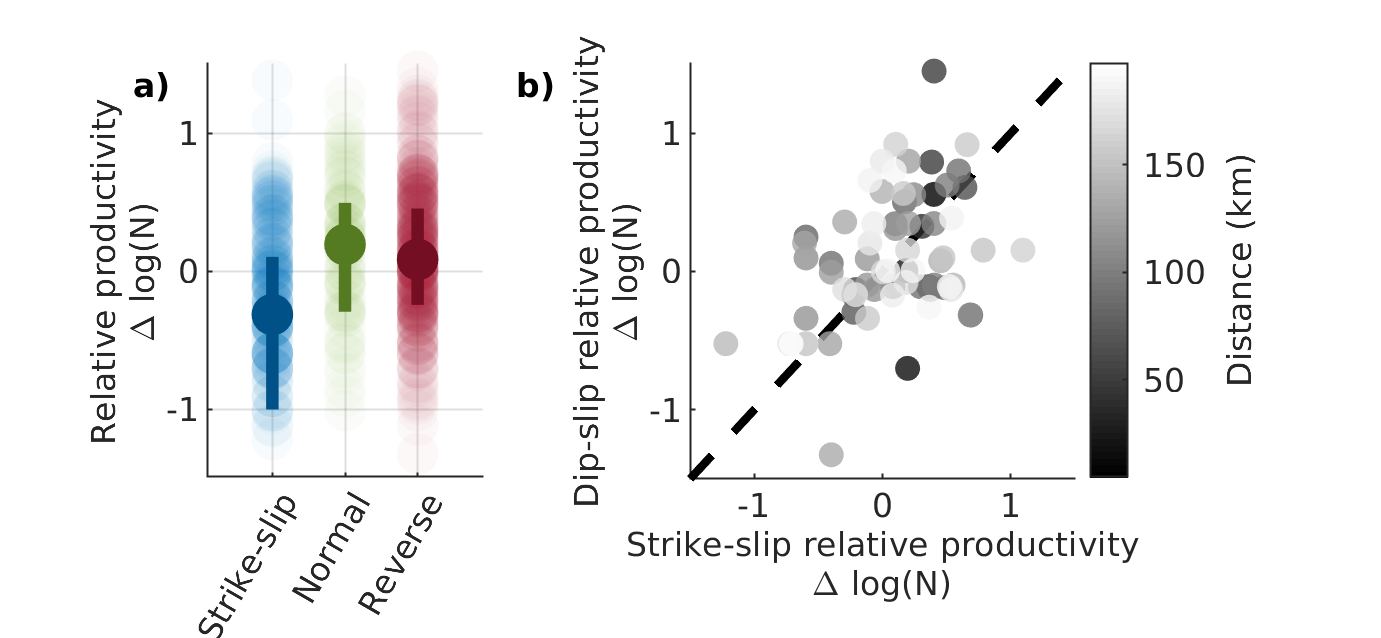
\includegraphics{figures/fmspairs.png}
        \caption{a) Relative aftershock productivity ($\Delta \log(N)$ by focal mechanism (Equation \ref{eq:residual_productivity}). b) Relative aftershock productivity for pairs of earthquake sequences with strike-slip and dip-slip mainshocks within 200 km from each other. Each pair is shaded according to its relative distance. Dashed line indicates a 1:1 relationship, the expectation for a purely site dominated control on relative productivity. Co-located mainshocks pairs generally follow this 1:1 trend, but exhibit considerable scatter.}
        \label{fig:coloc}
    \end{figure}
        
    \subsection{A Multi-Attribute Prediction of Aftershock Productivity}
    
    We have considered variables on a case by case basis and have prescribed a functional form to the relationships. In this section, we allow for increased complexity by utilizing machine learning tools to predict relative productivity given contextual information about the mainshocks setting and kinematics.
    
    As a point of reference, we produce predictions of relative productivity based on local seismicity. In this approach, aftershock productivity is predicted based on the median relative productivity of the ten nearest mainshocks. The chosen number of nearest neighbors produces the best predictions. Model validation is shown in Figure \ref{fig:response}a. This approach captures geographical effects and serves as a baseline for the following.
    
    We then tabulate earthquakes for which all parameters exist and systematically test predictions based permutations of parameters on various machine learning algorithms. To avoid over-fitting the data, we perform leave-one-out cross-validation---individual predictions are calibrated on the remainder of the data \citep{witten2011}. Support Vector Machines (SVM) yield the best predictions (Figure \ref{fig:response}b). Support vector machines aim to find lines, planes, or hyperplanes, that maximize the margins of the data by mapping data to higher dimensional spaces with transformations called kernels. Quadratic and cubic kernels produce similar results. SVMs are robust to over-fitting data and are therefore well suited for small datasets \citep{witten2011}. 
    
    The following metrics yield the best predictions of relative productivity: scaled rupture area, fault dip, and plate age. Better predictions on training data, with adverse predictions on the validation data, indicate that additional parameters do not improve predictions and instead induce over-fitting. The root mean squared error of the final model predictions of the SVM is 0.39, a 40\% improvement on the global productivity law and a 20\% improvement on the nearest neighbor algorithm, despite employing no direct geographical information. Of note, the SVM model better predicts extreme cases (highly productive or unproductive). The root mean squared error of the SVM is strongly influenced by the following two largest outliers, the 2017 $M_W7.0$ Loyalty Islands earthquake and the 2013 $M_W7.8$ Scotia Sea earthquake. Interestingly, both these mainshocks were preceded large foreshocks: two $M_W6+$ earthquakes for the former and a $M_W6.8$ earthquake for the latter. Removing these two outliers yields an additional 16\% improvement to the predictions.
    
    \begin{figure}
        \centering
        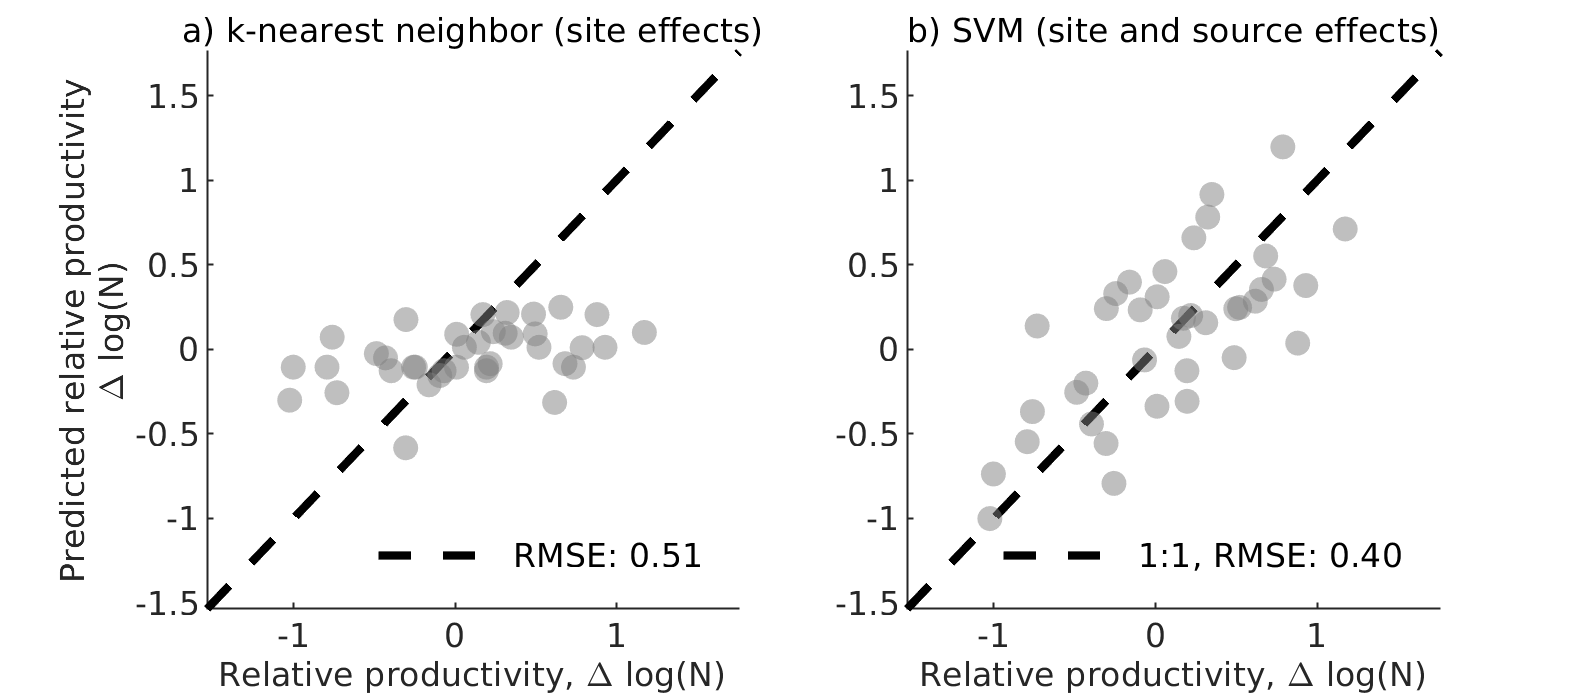
\includegraphics{figures/response.png}
        \caption{Response plots (prediction versus observation) for the k-nearest neighbor algorithm (a) and SVM models (b). Each point indicates prediction of relative productivity relative to that which was observed for individual earthquake sequences. A perfect prediction would place all values on the 1:1 line. The SVM model outperforms the k-nearest neighbor model. Combining both contextual information about the setting (crustal age) and the source (dip and normalized area) yields a root mean square value of 0.39.}
        \label{fig:response}
    \end{figure}
    
The preferred parameters of the SVM can be compared to those found in section \ref{sec:source_parameters}. For instance, dip appears to be more important in the SVM case. Aftershock productivity relates to dip non-monotonically with a maximum at intermediate  dips ($\sim 25^o$) (See Figure S12, Panel l). The added non-linearity allowed by the SVM model kernels is useful in this situation. Normalized rupture area is also more important in the SVM than in the linear regressions. This cause of this difference is harder to discern, but is likely a combination of the added non-linearity allowed by the SVM model and the co-variance across the combined attributes. These differences emphasize that the collapse of multivariate data into single attribute linear relationships has its limitations.

 \citet{Wetzler2016} interpreted higher stress drops to correlate with lower productivity as a result of a geometric effect. Higher stress drop means more compact rupture. Intriguingly, the simpler metric that focuses strictly on the geometric extent of the rupture appears to perform better than stress drop as an aftershock predictor in the SVM model. The normalized rupture area is a more direct measure of this physical relationship and appears to outweigh the effects of slip heterogeneity reflected in stress drop.

   %Normalized area anti-correlates with stress drop, yet it did not correlate well with relative productivity in the single attribute correlation. The difference in SVM and linear regression results may be do in part to the stronger selection criteria used for the SVM, resulted in a smaller dataset with different statistical properties. Elevated stress drop ruptures tend to occur in oceanic lithosphere \citep{choy2004apparent}, so that, within the more limited data set for which oceanic ages are available, the relationship is different. 
   
    %Redoing Figure~\ref{} with this smaller dataset results in normalized area  equivalent variance reduction for both parameters. Intriguingly, the simpler metric that focuses strictly on the geometric extent of the rupture appears to perform better as an aftershock predictor.

\section{Interpretation}

\subsection{Relative Importance of Setting and Source Effects}

We find that relative productivity is sensitive to both setting and source effects. From setting, dominant factors are lithospheric age, lithosphere type (oceanic vs. continental) and depth; from source, factors are area, aspect ratio and stress drop. Focal mechanism is an additional factor that can be construed as stemming from both tectonic setting and source. Figure \ref{fig:caltech} synthesizes these results demonstrating how significant factors compare to each other.
    
Our parameterization of slip heterogeneity does not correlate well with productivity. This observation contradicts some modelling predictions \citep{Helmstetter2006RelationModel, Marsan2006} and long-standing interpretations \citep{Mogi1967}. The observation suggests that the number of observable aftershocks is dominated by surrounding volume outside the main slip zone and less strongly modulated by residual stress on the fault plane \citep[as would be consistent with][]{Wetzler2018SystematicEarthquakes}. 
    
Measurements of relative productivity show no correlation with the scaled radiated energy of the mainshock. We gather that within three source dimensions of the mainshock static and quasi-static effects dominate earthquake triggering.
    
Comparing source and setting influences (Figure \ref{fig:caltech} emphasizes the role of the setting. The source parameters we consider tend to have a more subdued influence on the relative productivity (as shown in Figure \ref{fig:caltech}) than do some of the tectonic controls. Source attributes strongly co-vary with each-other; a possible consequence is that competing effects tend to subdue each-other. For instance, high stress drop ruptures drive more elevated stresses at the periphery of the fault which may contribute to higher aftershock productivity; but, this effect is reversed by the size of the rupture fault which is smaller for a high stress drop rupture \cite{Scholz2019}. Such competing effects might include predictions of elevated aftershock productivity associated with more energetic ruptures balanced by their occurrence in unproductive tectonic environments (e.g. oceanic lithosphere), predictions that more heterogeneous ruptures should be more productive offset by an association with higher stress drop compact ruptures. An exhaustive assessments of these and other causal relationships is beyond the scope of this study.
   
 \begin{figure}
        \centering
        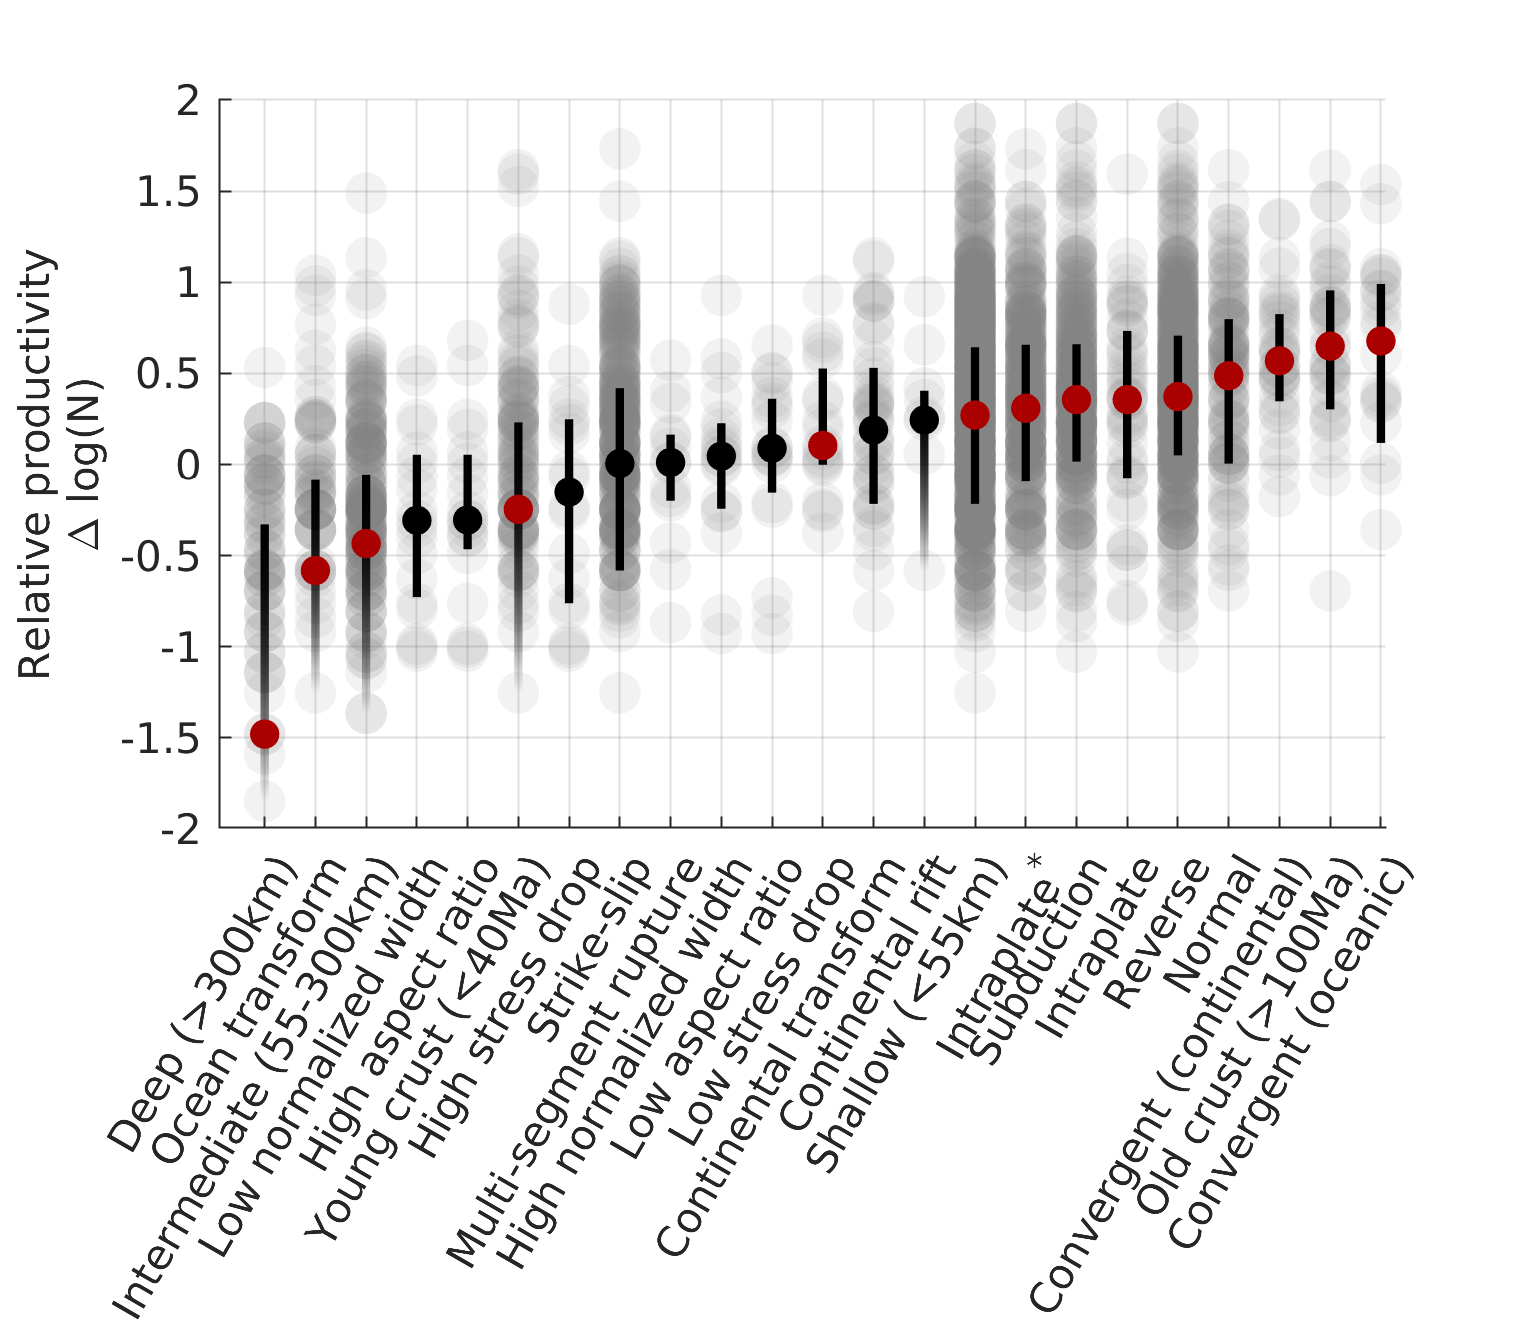
\includegraphics{figures/cal_tech.png}
        \caption{Synthesis of relative productivity according to catalog subsets. The group considered here are the short list which best distinguished relative productivity based on our different lines of investigation (Sections \ref{sec:glob}-\ref{sec:source_parameters}). `High' and `low' subsets respectively refer to $>80$th and $<20$th percentile ranges of the data. Grey circles are individual mainshocks. Black points and error bars respectively indicate the median and interaquartile range of the subset. Fading error bars imply that mainshock sequences with no aftershocks are within the interquartile range of the data.}
        \label{fig:caltech}
    \end{figure}   
    
    
\subsection{Importance of Fault Availability}

The dependence on crustal age, lithosphere type, depth, aspect ratio, stress drop, and the underlying magnitude scaling are all congruent with a single physical control: the primary influence on aftershock productivity is the available volume of rock susceptible to brittle failure. This consistency is perhaps the most significant result of this study.

The increase in earthquake productivity with plate age is, to the best of our knowledge a new finding. Figure \ref{fig:caltech} places this effect as the most pronounced control on aftershock statistics following depth effects. With increasing age, oceanic lithosphere becomes colder, thicker, more brittle and less buoyant. Subduction zone earthquakes hosted along younger lithosphere tend to generate larger earthquakes (lower b-values), particularly so in the first $\sim70$ Ma. \citet{Nishikawa2014EarthquakeBuoyancy} attributed the trend to changes in buoyancy of the subducting slab. While variations in b-value statistics may covary with aftershock productivity, we find it difficult to reconcile their physical interpretation with the increasing aftershock productivity along transform faults that we observe. Old oceanic lithosphere is also thicker. Increasing the thickness of the lithosphere increases the volume in the brittle failing regime. Increasing the susceptibility of the surrounding volume to earthquakes stressing is a natural alternative explanation for the increased rate of aftershocks with plate age. Though the effect was more subdued, a careful analysis of subduction zones also revealed the same pattern \citep[Appendix of][]{Wetzler2016}. Old ($>100Ma$) oceanic lithosphere hosts seismicity along Japan and in the western Mediterranean Sea, which are highly productive in aftershocks (see Figure \ref{fig:global_res} for reference). Generally, the contrasting aftershock productivity of the Eastern and Western Pacific can be related to lithospheric age. 

We may cast continental earthquakes, which we observe to have elevated aftershock productivity, as a highly thickened (old) lithosphere end member.  Equivalently, convergent boundaries which effectively double the thickness of the lithosphere are associated with high aftershock productivity. The deeper the zone of low temperature brittle material, the higher the aftershock production.

Intermediate- and deep-focus earthquakes are the opposite end-member, instead exhibiting very low aftershock productivity. Deep earthquakes within subducting oceanic lithosphere are confined above and below by viscous mantle. Moreover the the lithosphere is caused to thin by thermal conduction from the warmer mantle. Subducting lithosphere becomes rejuvenated and hence aftershock poor.

Long aspect ratio ruptures reflect the saturation of the brittle crust --- in this case, above by the surface of the Earth and below by viscous dissipation \citep{Scholz2019}. Spatial confines limit the volume that may host aftershocks. It is telling to observe that the down-dip width of the rupture correlates far better with aftershock productivity than its the length (Figure \ref{fig:r2_finite_fault}). In other words, vertical confines (the surface and the ductile base of the seismogenic zone) are better controls on the productivity of earthquakes than the lateral limits. 

The final evidence for the significance of volume availability arises from the scaling of aftershocks productivity with mainshock size. The scaling captures the mainshocks ability to activate a larger volume with increasing earthquake size. Our results are a natural extension of this basic premise. Fluctuations to the magnitude scaling, i.e. relative productivity, result from fluctuations in mainshocks ability to brittlely deform its surrounding volume. 
    
\subsection{Improving Aftershock Prediction}
 
Short term hazard assessment following a large earthquake relies on regional catalogs to calibrate the statistical behavior of the seismicity. Unfortunately, seismic records are temporally limited and generally do not span large-earthquake-cycle timescales, particularly for the determination of aftershock parameters such as aftershock productivity. Expert predictions, therefore, will often rely on past ruptures that may serve as analogs for the upcoming hazard. We extend this approach with a statistical treatment using flexible prediction tools. Using local analogs to determine the aftershock hazard is often impossible. Our analysis raises an alternative approach. We show that contextual attributes are strongly indicative of upcoming aftershock productivity. Therefore, teleseismic data and knowledge of the local tectonic context can help constrain short-term hazard following large earthquakes in poorly instrumented or quiescent areas. In particular, Figure \ref{fig:response}b suggests an algorithm to use in future aftershock prediction.

\section{Conclusion}

We synthesize multiple possible relationships between aftershock productivity and setting/source effects for earthquakes from 1990 to 2019. Global patterns suggest that earthquake productivity is particularly low along oceanic transform faults and tracks lithosphere ages. The functional relationship suggests that productivity increases because of the cooling and thickening of oceanic lithosphere with time. The rupture's aspect ratio, the down-dip width and, to a lesser degree, stress drop, correlate with aftershock productivity; other parameters including rupture duration, and length, scaled radiated energy and material parameters did not. Just a few parameters (plate age, dip, and normalized rupture area) are promising predictors of short-term seismicity forecast. Predictions do not require knowledge of the regional seismicity and therefore lend themselves well to large remote earthquakes where teleseismic data is available, but long term monitoring is not. Source geometry and the availability of stressed faults are inferred to provide primary control on the number of aftershocks triggered.

\acknowledgments
We would like to thank the all members of the UCSC seismology laboratory for providing thoughtful insight and lively debate on the topic. Earthquake locations and magnitudes along with estimates of radiated energy were obtained were retrieved from the IRIS data management center. Gavin Hayes provided all finite fault inversions. To the best of our knowledge, no author has any conflict of interest publishing this research.

\bibliography{references.bib}

\end{document}
